\hypertarget{ll__flush_8c}{
\section{ll\_\-flush.c File Reference}
\label{ll__flush_8c}\index{ll_flush.c@{ll\_\-flush.c}}
}


\subsection{Detailed Description}
\begin{Desc}
\item[For internal use only.]
This file contains the implementation of the \hyperlink{group__dbprim__link_ga11}{ll\_\-flush()} function, used to remove every element from a linked list.\end{Desc}


Definition in file \hyperlink{ll__flush_8c-source}{ll\_\-flush.c}.

{\tt \#include \char`\"{}dbprim.h\char`\"{}}\par
{\tt \#include \char`\"{}dbprim\_\-int.h\char`\"{}}\par


Include dependency graph for ll\_\-flush.c:\begin{figure}[H]
\begin{center}
\leavevmode
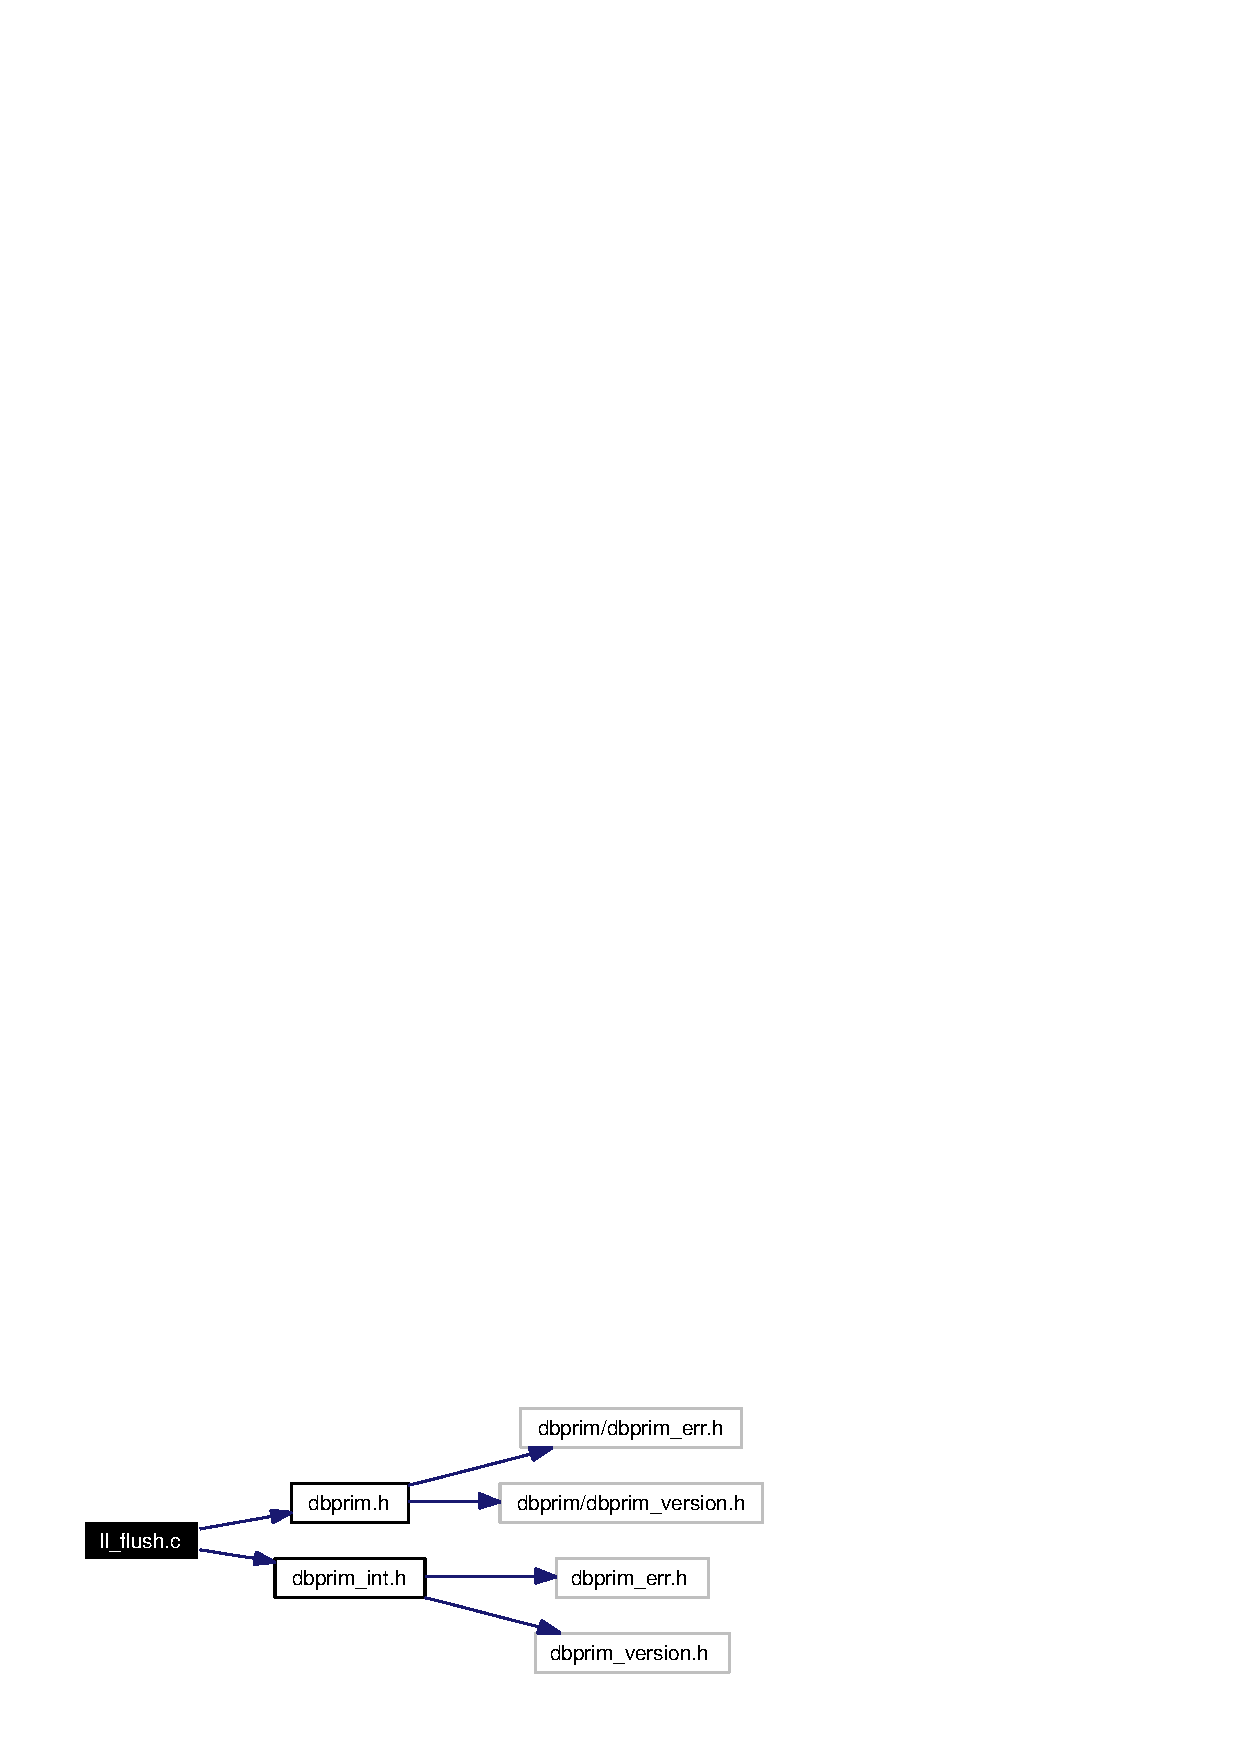
\includegraphics[width=185pt]{ll__flush_8c__incl}
\end{center}
\end{figure}
\subsection*{Functions}
\begin{CompactItemize}
\item 
unsigned long \hyperlink{group__dbprim__link_ga11}{ll\_\-flush} (\hyperlink{struct__link__head__s}{link\_\-head\_\-t} $\ast$list, \hyperlink{group__dbprim__link_ga2}{link\_\-iter\_\-t} flush\_\-func, void $\ast$extra)
\begin{CompactList}\small\item\em Flush a linked list. \item\end{CompactList}\end{CompactItemize}
